\documentclass[]{report}

\voffset=-1.5cm
\oddsidemargin=0.0cm
\textwidth = 480pt

\usepackage{framed}
\usepackage{subfiles}
\usepackage{enumerate}
\usepackage{graphics}
\usepackage{newlfont}
\usepackage{eurosym}
\usepackage{amsmath,amsthm,amsfonts}
\usepackage{amsmath}
\usepackage{color}
\usepackage{amssymb}
\usepackage{multicol}
\usepackage[dvipsnames]{xcolor}
\usepackage{graphicx}
\begin{document}
	
%------------------------------------%
\chapter{Session 6}
\section*{Session 06: Digraphs and Relations}
\begin{itemize}
\item[6A.1] In-degree and out-degree
\item[6A.2]
\item[6A.3]
\end{itemize}
\subsection*{Relations}
\begin{itemize}
\item[6B.1] Equivalence RElations (6.2.2)
\item[6B.2]
\item[6B.3] Relations and Cartesian Products (6.3)
\end{itemize}


\begin{itemize}
\item \textbf{Reflexive}: 
\item \textbf{Symmetric}: 
\item \textbf{Transitive}: 
\item \textbf{Anti-symmetric}: 
\item \textbf{Equivalence Relation}: 
\item \textbf{Partial Order}:
\item \textbf{Order}:
\end{itemize}

%-----------------------------------------------------%
\section*{Question 6}

\subsection*{Part A : Digraphs}

Suppose $A = \{1,2,3,4\}$. Consider the following relation in A

\[ \{  (1,1),(2,2),(2,3),(3,2),(4,2),(4,4)\} \]

Draw the direct graph of $A$. Based on the Digraph of $A$ discuss whether or not a relation that could be depicted by the digraph could be described as the following, justifying your answer.


\begin{itemize}
\item[(i)] Symmetric
\item[(ii)] Reflexive 
\item[(iii)] Transitive
\item[(iv)] Antisymmetric
\end{itemize}
\subsection*{Part B : Relations}
Determine which of the following relations $ x R y$ are reflexive, transitive, symmetric, or antisymmetric on the following - there may be more than one characteristic.  if

\begin{itemize} 
\item[(i)] $x = y$
\item[(ii)] $x < y$
\item[(iii)] $x^2 = y^2$
\item[(iv)] $x \geq y$
\end{itemize}
\subsection*{Part C : Partial Orders}
% http://staff.scem.uws.edu.au/cgi-bin/cgiwrap/zhuhan/dmath/dm_readall.cgi?page=20

Let $A=\{0,1,2\}$ and $R=\{ (0,0),(0,1),(0,2),(1,1), (1,2), (2,2)\}$
and $S=\{(0,0),(1,1),(2,2)\}$ be 2 relations on A. Show that

\begin{itemize}
\item[(i)] R is a partial order relation.
\item[(ii)] S is an equivalence relation.
\end{itemize}



\section{Digraphs and Relatiosn}
% 2007 Q8
Given a flock of chickens, between any two chickens one of them is
dominant. A relation, R, is defined between chicken x and chicken y as xRy if x is
dominant over y. This gives what is known as a pecking order to the flock. Home
Farm has 5 chickens: Amy, Beth, Carol, Daisy and Eve, with the following relations:

\begin{itemize}
\item Amy is dominant over Beth and Carol
\item Beth is dominant over Eve and Carol
\item Carol is dominant over Eve and Daisy
\item Daisy is dominant over Eve, Amy and Beth
\item Eve is dominant over Amy.
\end{itemize}

\newpage

\chapter{Session 7}

%------------------------------------%

\section*{Session 07:Sequences and Series}
\begin{itemize}
\item[7A.1] Sequences
\item[7A.2] Induction
\item[7A.3] Series and the Sigma Notation
\end{itemize}

\subsection*{Recurrence Relations(7.1.1)}



$u_1 = 2$
$u_2 = u_1 + 3 = 2 +3 = 5$
$u_3 = u_2 + 3 = 5+ 3 = 8$
Airthmetic Progression


\subsection*{Proof by Induction(7.2.2)}
\begin{itemize}
\item[Step 1] Base case
\item[Step 2] Induction hypothesis
\item[Step 3] Induction step
\end{itemize}



\subsection*{Series and Sigma Notation(7.2.3)}


%-----------------------------------------------------%

\section*{Question 7}
\subsection*{Part A : Recurrence Relations}
A sequence is defined by the recurrence relations
\[x_{n+2}  = 3x_{n+1} - 2x_n\]
with initial terms $x_1 = 1$ and $x_2=3$.

\begin{itemize}
\item[(i)] Calculate $x_3$, $x_4$ and $x_5$, showing your workings.
\item[(ii)] Prove by induction that $x_n = 2^n - 1$ for all $n \geq 1$
\end{itemize}

%------------------------------------%
\subsection*{Part B : Summations}

Compute the following summation

\[ \sum^{i=100}_{i=25} i^2 + 3i -5)\]
%------------------------------------%


Say which of the set the following numbers belong to.

If they belong to more than one of these sets, give all the sets.

$\sqrt{2}$
$\frac{3}{7}$

%------------------------------------------------------



\subsection*{Section 8 Exercises}
\begin{itemize}
\item $8^{\frac{1}{3}}$ Recall $a^{\frac{b}{c}} = a^{\frac{b}{c}}$
\item
\item
\end{itemize}




%------------------------------------%

\section*{Question 7b}

Compute the following summation

\[ \sum^{i=100}_{i=25} i^2 + 3i -5)\]


%------------------------------------%

\section*{Question 7}
A sequence is defined by the formula 
$u_n = 5n-3$ for $n\geq 1$

\[\frac{n(n+1)(2n+1)}{6}\]

Write the following sums in the $\Sigma$ notation and evaluate them

\begin{itemize}
\item $1^2 + 2^2 + 3^2 +  \ldots +  40^2 = ?$
\item $2 + 5 + 10 + \ldots + 1601 = ?$
\item $2+8+18+\ldots +3200 = ?$
\end{itemize}

\section*{Part A : Recurrence Relations}
A sequence is defined by the recurrence relations
\[x_{n+2}  = 3x_{n+1} - 2x_n\]
with initial terms $x_1 = 1$ and $x_2=3$.

\begin{itemize}
\item[(i)] Calculate $x_3$, $x_4$ and $x_5$, showing your workings.
\item[(ii)] Prove by induction that $x_n = 2^n - 1$ for all $n \geq 1$
\end{itemize}

%------------------------------------%




\section*{Proof By Induction}

\begin{itemize}
\item \textbf{Base Step}
\item \textbf{Induction Step}
\item \textbf{Some Step}
\end{itemize}

%------------------------- %
%-------------------------- %

%------------------------------------%
\subsection{Sequence and Series and Proof by Induction}


\[\sum^{n}_{i=1} (n^2) \]


\section{Proof By Induction}

Prove by Induction the following expression
\[ \sum_{r=1}^{r=n} r^2 = \frac{n(n+1)(2n+1)}{6} \]
for all $n \in N_0$.


\begin{itemize}
	\item \textbf{Step 1} : Is the proposition true for $n = 1$?
	\item \textbf{Step 2} : Show that if the proposition is true for $n=k$, then it is also true for $n=k+1$.
	\item \textbf{Step 3} : Conclude that the proposition is true for all natural numbers greater than or equal to one.
\end{itemize}

%------------------------------------------------ %

\subsection{Proof By Induction}

Prove by induction the following expression
\[ \sum_{r=1}^{r=n} r^2 = \frac{n(n+1)(2n+1)}{6} \]
for all $n \in N_0$.
\begin{itemize}
	\item \textbf{Step 1} : Is the proposition true for $n = 1$? 
\end{itemize}
\textbf{Left-hand side}
\[ \sum_{r=1}^{r=1} r^2 = 1^2 = 1 \]



\textbf{Left-hand side}
\[ \sum_{r=1}^{r=1} r^2 = 1^2 = \boldsymbol{1} \]
\textbf{Right-hand side}

\[ \frac{n(n+1)(2n+1)}{6}  = \frac{1(1+1)(2\cdot 1+1)}{6} \]
\[  = \frac{1\times 2 \times 3}{6} = \frac{6}{6}=\boldsymbol{1} \]

%------------------------------------------------ %


\begin{itemize}
	\item \textbf{Step 1} : Is the proposition true for $n = 1$? 
\end{itemize}
\bigskip
Yes: The left-hand side and right-hand side of the equation yield the same value.

\begin{itemize}
	\item \textbf{Step 2} : Show that if the proposition is true for $n=k$, then it is also true for $n=k+1$.
\end{itemize}
Given: \[ \sum_{r=1}^{r=k} r^2 = \frac{k(k+1)(2k+1)}{6} \]

To Prove: \[ \sum_{r=1}^{r=k+1} r^2 = \frac{(k+1)(k+2)(2k+3)}{6} \]


%------------------------------------------------ %

\subsection{Proof By Induction}
%% - \vspace{-1cm}



\[ \sum_{r=1}^{r=k+1} r^2 = 1^2 + 2^2 + 3^2 + \ldots + k^2 + (k+1)^2 \]






\[ \sum_{r=1}^{r=k+1} r^2 = 1^2 + 2^2 + 3^2 + \ldots + k^2 + (k+1)^2 \]

\[ \sum_{r=1}^{r=k+1} r^2 = \boldsymbol{\sum_{r=1}^{r=k} r^2} + (k+1)^2 \]



\[ \sum_{r=1}^{r=k+1} r^2 = \boldsymbol{\sum_{r=1}^{r=k} r^2} + (k+1)^2 \]

\[ \sum_{r=1}^{r=k+1} r^2 = \frac{k(k+1(2k+1
	))}{6} + (k+1)^2 \]


%---------------------------------------%
\chapter{Session 8}
% % Section 8 Trees
%-----------------------------------------------------%
\section*{Question 8}
\subsection*{Part A : Spanning Trees}
\begin{enumerate}
\item How many edges are in the spanning tree $T$ ?
\item What is the sum of the degree sequence of $T$?
\item Write down all the possible degree sequences for the spanning tree $T$.
\end{enumerate}
%------------------------------------%

\subsection*{Part B : Binary Search Trees}
Suppose a database, comprised of 30,000 internal nodes, is structured as a Binary Search Tree.

\begin{enumerate}
\item What is the key (number) of the Root node?
\item What are the keys of the nodes at level 1?
\item For the nodes at level1, how many subtrees are there?
\item State which nodes are in the substrees of the level 1 nodes?
\item How many nodes are the between the root (level 0) and level 7. ]
(Hint: use a summation theorem mentioned in session 7
\item What is the maximum number of searchs in this database?
\end{enumerate}




\section{Question 8B}
Suppose a database, comprised of 30,000 internal nodes, is structured as a Binary Search Tree.

\begin{enumerate}
\item What is the Key of the Root node?
\item What are the keys of the nodes at level 1?
\item For the nodes at level1, how many subtrees are there?
\item State which nodes are in the substrees of the level 1 nodes?
\item How many nodes are the between the root (level 0) and level 7. ]
(Hint: use a summation theorem mentioned in session 7
\item What is the maximum number of searchs in this database?
\end{enumerate}
%--------------------------------------------------------------------

\section*{Binary Search Trees}
What is a Binary Search Tree
\[ \lfloor  \frac{\mbox{log}_2}{T} \rfloor \]

%------------------------- %
%-------------------------- %
\section*{Session 08:Trees}
\begin{itemize}
\item[8A.1] Trees
\item[8A.2] Spanning Trees
\item[8A.3] Rooted trees
\item[8A.4] Binary Search Trees
\end{itemize}
A tree is a directed graph that contains no cycles.
%-----------------------------------------------------%
\section{Question 8}

1) Draw this tree
2) Construct all the isomorphic tress with 6 vertices which can be obtainbed by attaching a new vertex of degreee one to a vertex of T.
3) Explain briefly why the tree obtained in (ii) is not isomorphic to each other.
4) Construct a tree with 6 vertices which is not isomorphic to any tree you constructed in (ii)

Part b
Determine the number of nodes on level 5 and level 10
Find an expression in terms of $\Sigma$ and h for the number of internal nodes in such a tree.
What is the smallest possible height of such a tree if there are at least 900 internal nodes.

% %------------------------------------------------------

\section{Question 8A}
\begin{enumerate}
\item How many edges are in the spanning tree $T$ ?
\item What is the sum of the degree sequence of $T$?
\item Write down all the possible degree sequences for the spanning tree $T$.
\end{enumerate}

\section{Tree Definition}
What properties must a graph have in order for it to be a
tree?
(ii) Say, with reason, whether or not it is possible to construct a tree with
degree sequence 4, 3, 3, 1, 1.
\newpage

\subsection*{Question 1}

(b) Express the following hexadecimal number as a decimal number: (A32.8)16.
[3]
(c) Convert the following decimal number into base 2, showing all your working:
$(253)_{10}$. [2]
(d) Express the recurring decimal $0.4242424\ldots$
as a rational number in its simplest
form. [2]


%---------------------------------------%
\subsection*{Question 7}
%2002 Question 7
Let S be a set and let R be a relation on S
Explain what it means to say thet $\mathcal{R}$ is

\begin{itemize}
	\item[(i)] reflexive
	\item[(ii)] symmetrix
	\item[(iii)] anti-symmetric
	\item[(iv)] Transitive
\end{itemize}


\subsection{Question 10}

(a) Given the following adjacency matrices A and B where
A =

1 0 1
0 1 2
1 2 0

,B =

1 2 0
2 0 1
0 1 1

%MAKE NO

%--------------------------------------------%

(i) Say whether or not the graphs they represent are isomorphic.
(ii) Calculate A2 and A4 and say what information each gives about the graph
corresponding to A. [6]
(b) (i) Write down the augmented matrix for the following system of equations.

\[2x + y - z = 2\]
\[x - y + z = 4\]
\[x + 2y + 2z = 10\]
(ii) Use Gaussian elimination to solve the system. [4]


%--------------------------------------------%
\newpage
\chapter{Session 9}
\section{Probability and Counting}

% 2007 Q8
Given S is the set of all 5 digit binary strings, E is the set of a 5 digit
binary strings beginning with a 1 and F is the set of all 5 digit binary strings ending
with two zeroes.
\begin{itemize}
\item[(a)] Find the cardinality of S, E and F.
\item[(b)] Draw a Venn diagram to show the relationship between the sets S, E and F.
\item[(c)]Show the relevant number of elements in each region of your diagram.
\end{itemize}
%-------------------------------------------------------------------------%
\newpage


\begin{frame}
\frametitle{Proof By Induction}
\Large
\textbf{Three Steps}
\begin{description}
\item[Step 1]
\item[Step 2]
\item[Step 3]
\end{description}

\end{frame}
%-------------------------------------------------------------------%
\begin{frame}
\frametitle{Proof by Induction}
\Large
Let the summation $s_n$ be defined as follows:
\[s_n = 1 + 3 + 5 + \ldots + (2n - 1) \qquad \mbox{for n }\in \mathbb{Z}^{+}\]

Use the method of induction to prove that $s_n = n^2$ for all $n \geq 1$.
\end{frame}

%------------------------------------------- %


%------------------------- %
% Section 1
\subsection{Axioms of Probability}

The Axioms of Probability

\begin{itemize}
\item The probability of a certain event is 1.
\item The probability of an impossible event is 0.
\item 
\end{itemize}
%------------------------- %
%-------------------------- %
\section*{Session 09: Probability}
\begin{itemize}
\item[9A.1] Counting Methods
\item[9A.2] Counting using Sets
\item[9A.3] Probability
\item[9A.4] Independent Events
\end{itemize}
\begin{itemize}
\item[9B.1] Permutation

\[ {n \choose r} = \frac{n!}{(n-r)! r!} \]


\[ {6 \choose 3} = \frac{6!}{(6-3)! 3!} = \frac{6!}{3! \times 3!}\]


\[ \frac{6!}{3! \times 3!} = \frac{6 \times 5 \times 4 \times 3!}{3! \times 3!} = \frac{120}{6} = 120\]
\end{itemize}
%\begin{multicol}{2}
\begin{itemize}
\item ${6 \choose 2} = 15$
\item ${5 \choose 2} = 10$  
\item ${4 \choose 0} = 1$  
\item ${4 \choose 3} = 4$  
\end{itemize}
%\end{multicol}

\begin{itemize}
\item pairwise disjoint sets
\item The addition principle
\end{itemize}
\subsection*{Theorem}
\[ |A \cup B| = |A| + |B| - |A \cap B|  \]

\subsection*{Probability}
\begin{itemize}
\item[9B.2] The sample space of an experiment ($S$)
\item[9B.3] The size of a sample space
\item[9B.4] Indepedent Evcents (9.3.1)
\end{itemize}
%-----------------------------------------------------%

\chapter{Permutations}

%-------------------------------------%
\begin{frame}
\frametitle{Permutations}
\Large
\vspace{-2cm}
How many anagrams (permutations of the letters) are there of the following words
\begin{enumerate}
\item ANSWER
\item PERMUTE
\item ANAGRAM
\item LITTLE
\end{enumerate}

\end{frame}
%-------------------------------------%
\begin{frame}
\frametitle{Permutations}
\Large
\vspace{-2cm}
\textbf{Part 1 : ANSWER}\\
Examples:
\begin{center}
ASNWRE,\;
SANERW,\;
REWSAN,\;...
\end{center}

Since ANSWER has 6 distinct letters, the number of permutations (anagrams) is
\LARGE
\[6! = 6\times 5 \times 4 \times 3 \times 2\times 1 = \boldsymbol{720} \]
\end{frame}
%-------------------------------------%
\begin{frame}
\frametitle{Permutations}
\Large
\vspace{-0.3cm}
\textbf{Part 2 : PERMUTE}\\
\begin{itemize}
\item The word PERMUTE has 7 letters, but only 6 different letters. 
\item There are 7! ways to arrange 7 letters.
\item However, interchanging the two Es does not result in a new permutation. There would be two identical anagrams.
\end{itemize}

\begin{center}
P\textcolor{red}{E}RMUT\textcolor{blue}{E}, \; MUT\textcolor{red}{E}P\textcolor{blue}{E}R, \; P\textcolor{red}{E}T\textcolor{blue}{E}MUR,\; ..\\
P\textcolor{blue}{E}RMUT\textcolor{red}{E}, \; MUT\textcolor{blue}{E}P\textcolor{red}{E}R, \; P\textcolor{blue}{E}T\textcolor{red}{E}MUR,\; ..
\end{center}
\end{frame}
%-------------------------------------%
\begin{frame}
\frametitle{Permutations}
\Large
\vspace{-0.3cm}
\textbf{Part 2 : PERMUTE}\\
\begin{itemize}
\item The number of permutations (anagrams) is half of 7! .
\LARGE
\[\frac{7!}{2} =  \frac{5040}{2} = \boldsymbol{2520} \]
\end{itemize}
\end{frame}

%-------------------------------------%
\begin{frame}
\frametitle{Permutations}
\Large
\vspace{-0.1cm}
\textbf{Part 3 : ANAGRAM}\\
\begin{itemize}
\item The word ANAGRAM has 7 letters, but there are three As.
\item From before, there are 7! ways to arrange 7 letters.
\item How many new permutations are found by re-arranging the As?
\end{itemize}
\LARGE
\begin{center}
\textcolor{red}{A}N\textcolor{blue}{A}GR\textcolor{purple}{A}M \; 
\textcolor{red}{A}N\textcolor{purple}{A}GR\textcolor{blue}{A}M \; 
\textcolor{blue}{A}N\textcolor{red}{A}GR\textcolor{purple}{A}M \; \\
\textcolor{purple}{A}N\textcolor{red}{A}GR\textcolor{blue}{A}M \; 
\textcolor{blue}{A}N\textcolor{purple}{A}GR\textcolor{red}{A}M \; 
\textcolor{purple}{A}N\textcolor{blue}{A}GR\textcolor{red}{A}M \; 
\end{center}
\end{frame}

%-------------------------------------%
\begin{frame}
\frametitle{Permutations}
\Large
\vspace{-0.1cm}
\textbf{Part 3 : ANAGRAM}\\
\begin{itemize}
\item We divide 7! by 3! to account for the identical anagrams.
\LARGE
\[\frac{7!}{3!} =  \frac{5040}{6} = \boldsymbol{840} \]
\end{itemize}
\end{frame}
%-------------------------------------%
\begin{frame}
\frametitle{Permutations}
\Large
\vspace{-2.3cm}
\textbf{Part 2 : PERMUTE}\\
\begin{itemize}
\item We re-express the answer from part 2 as follows:
\LARGE
\[\frac{7!}{2!} =  \frac{5040}{2} = \boldsymbol{2520} \]
\end{itemize}
\end{frame}
%-------------------------------------%
\begin{frame}
\frametitle{Permutations}
\Large
\vspace{-0.3cm}
\textbf{Part 4 : LITTLE}\\
\begin{itemize}
\item The word LITTLE has 6 letters, but there are two Ls and two Ts.
\item From before, there are 6! ways to arrange 6 letters.
\item Again, interchanging the two Ls and Ts does not result in a new permutation. 
\LARGE
\[\frac{6!}{2!\times 2!} =  \frac{720}{4} = \boldsymbol{180} \]
\end{itemize}
\end{frame}
%------------------------------------------------%
\section*{Session 9 Probability}
\subsection*{Binomial Coefficients}
\begin{itemize}
\item factorials 
\[ n! = (n)\times (n-1)\times(n-2) \times \ldots \times 1 \]
\begin{itemize}
\item $5! = 5 \times 4 \times 3 \times 2 \times 1 = 120 $
\item $3! = 3 \times 2 \times 1$
\end{itemize}
\item Zero factorial
\[ 0! =  1 \]
\end{itemize}
%---------------------------------------------- %

% \[P(A |B = \frac{P(A \cap B)}{P(B)})\]

The complement rule in Probability

$P(C^{\prime}) = 1- P(C)$



If the probability of C is $70 \%$ then the probability of $C^{\prime}$ is $30\%$


%------------------------------------------------%
\section*{Probability}
\subsection*{Binomial Coefficients}
\begin{itemize}
\item factorials 
\[ n! = (n)\times (n-1)\times(n-2) \times \ldots \times 1 \]
\begin{itemize}
\item $5! = 5 \times 4 \times 3 \times 2 \times 1 = 120 $
\item $3! = 3 \times 2 \times 1$
\end{itemize}
\item Zero factorial
\[ 0! =  1 \]
\end{itemize}
%---------------------------------------------- %

% \[P(A |B = \frac{P(A \cap B)}{P(B)})\]

The complement rule in Probability

$P(C^{\prime}) = 1- P(C)$



If the probability of C is $70 \%$ then the probability of $C^{\prime}$ is $30\%$


\section{Counting}
% 2007 Q8
Given S is the set of all 5 digit binary strings, E is the set of a 5 digit
binary strings beginning with a 1 and F is the set of all 5 digit binary strings ending
with two zeroes.
\begin{itemize}
\item[(a)] Find the cardinality of S, E and F.
\item[(b)] Draw a Venn diagram to show the relationship between the sets S, E and F.
\item[(c)] Show the relevant number of elements in each region of your diagram.
\end{itemize}


\section*{Probability: Binomial Coefficients}
\begin{itemize}
\item factorials 
\[ n! = (n)\times (n-1)\times(n-2) \times \ldots \times 1 \]
\begin{itemize}
\item $5! = 5 \times 4 \times 3 \times 2 \times 1 = 120 $
\item $3! = 3 \times 2 \times 1$
\end{itemize}
\item Zero factorial
\[ 0! =  1 \]
\end{itemize}
%---------------------------------------------- %

% \[P(A |B = \frac{P(A \cap B)}{P(B)})\]

The complement rule in Probability

$P(C^{\prime}) = 1- P(C)$



If the probability of C is $70 \%$ then the probability of $C^{\prime}$ is $30\%$



%-------------------------------------------------------%
{
	{Basic Operations with Matrices  }
%-------------------------------------------------------%
{
	{Basic Operations with Matrices }
	
	\begin{itemize}
		\item Addition of Matrices
		\item Transpose of a Matrix
		\item Adding and Subtracting Matrices
		\item Scalar Multiplication
	\end{itemize}
}

%-------------------------------------------------------%
{
	
	{Matrix Multiplication}
	{
		
		\[ \left(
		\begin{array}{cc}
		a & b \\
		c & d \\
		\end{array}
		\right) \times \left(
		\begin{array}{cc}
		u & v \\
		w & x \\
		\end{array}
		\right)
		\]
		
		
		
		\[ \left(
		\begin{array}{cc}
		a & b \\
		c & d \\
		\end{array}
		\right) \times \left(
		\begin{array}{cc}
		u & v \\
		w & x \\
		\end{array}
		\right)
		\]
		
		
		
		\[ \left(
		\begin{array}{cc}
		3 & 1 \\
		2 & 4 \\
		\end{array}
		\right) \times \left(
		\begin{array}{cc}
		2 & 5 \\
		4 & 1 \\
		\end{array}
		\right)
		\]
		
		{Matrix Multiplication}
		
		{\huge
			
			\[ \left(
			\begin{array}{cc}
			\underline{\boldsymbol{a}}& \underline{\boldsymbol{b}} \\
			c & d \\
			\end{array}
			\right) \times \left(
			\begin{array}{cc}
			u & v \\
			w & x \\
			\end{array}
			\right)
			\]
			
			%-------------------------------------------------------%
			{
				{Matrix Multiplication}
				
				{\huge
				
						\[ \left(
						\begin{array}{cc}
						\boldsymbol{a} & \boldsymbol{b} \\
						c & d \\
						\end{array}
						\right) \times \left(
						\begin{array}{cc}
						\underline{\textcolor{green}{u}} & v \\
						\underline{\textcolor{green}{w}} & x \\
						\end{array}
						\right)
						\]
						
						
						{Matrix Multiplication}
						
						{\huge
							
							\[ \left(
							\begin{array}{cc}
							\boldsymbol{a} & \boldsymbol{b} \\
							c & d \\
							\end{array}
							\right) \times \left(
							\begin{array}{cc}
							\textcolor{green}{u} & v \\
							\textcolor{green}{w} & x \\
							\end{array}
							\right)
							\]
							
							\[ = \left(
							\begin{array}{cc}
							\boldsymbol{a}\textcolor{green}{u} + \boldsymbol{b}\textcolor{green}{w}& \ldots \ldots\\
							\ldots \ldots & \ldots \ldots \\
							\end{array}
							\right) 
							\]
							
	
	\textbf{Transpose of a Matrix}
	\begin{itemize}
		
		\item The transpose of a matrix is transformation of that matrix when all the rows are arranged into columns and columns arranged by rows.
		\item The transpose of a matrix $A$ is usually denoted $A^{T}$ or $A^{\prime}$.
		\item The relevant \texttt{R} function is \texttt{t()}.
	\end{itemize}

	{Sample Space (2)}
	Consider a random experiment in which a coin is tossed once, and a number between 1 and 4 is selected at random.
	Write out the sample space $S$ for this experiment.
	
	\bigskip
	
	\[ S = \{(H,1),(H,2),(H,3),(H,4),(T,1),(T,2),(T,3),(T,4)\} \]
	
	( $H$ and $T$ denoted `Heads' and `Tails' respectively. )
	
}
%-------------------------------------------------------%
{
	{Contingency Tables}
	Suppose there are 100 students in a first year college intake.  \begin{itemize} \item 44 are male and are studying computer science, \item 18 are male and studying statistics \item 16 are female and studying computer science, \item 22 are female and studying statistics. \end{itemize}
	\bigskip
	We assign the names $M$, $F$, $C$ and $S$ to the events that a student, randomly selected from this group, is male, female, studying computer science, and studying statistics respectively.
}
%-------------------------------------------------------%
{
	{Contingency Tables}
	The most effective way to handle this data is to draw up a table. We call this a \textbf{\emph{contingency table}}.
	\\A contingency table is a table in which all possible events (or outcomes) for one variable are listed as
	row headings, all possible events for a second variable are listed as column headings, and the value entered in
	each cell of the table is the frequency of each joint occurrence.
	
	
	\begin{center}
		\begin{tabular}{|c|c|c|c|}
			\hline
			% after \\: \hline or \cline{col1-col2} \cline{col3-col4} ...
			& C & S & Total \\ \hline
			M & 44 & 18 & 62 \\ \hline
			F & 16 & 22 & 38 \\ \hline
			Total & 60 & 40 & 100 \\ \hline
		\end{tabular}
	\end{center}
	
}
%-------------------------------------------------------%
{
	{Contingency Tables}
	It is now easy to deduce the probabilities of the respective events, by looking at the totals for each row and column.
	\begin{itemize}
		\item P(C) = 60/100 = 0.60
		\item P(S) = 40/100 = 0.40
		\item P(M) = 62/100 = 0.62
		\item P(F) = 38/100 = 0.38
	\end{itemize}
	\textbf{Remark:}\\
	The information we were originally given can also be expressed as:
	\begin{itemize}
		\item $P(C \cap M) = 44/100 = 0.44$
		\item $P(C \cap F) = 16/100 = 0.16$
		\item $P(S \cap M) = 18/100 = 0.18$
		\item $P(S \cap F) = 22/100 = 0.22$
	\end{itemize}
}

%-------------------------------------------------------%
{
	{Conditional Probability (1)}
	
	The definition of conditional probability:
	\[ P(A|B) = \frac{P(A \cap B)}{P(B)} \]
	
	\begin{itemize}
		\item $P(B)$ Probability of event B.
		\item [ $P(A)$ Probability of event A. ]
		\item $P(A|B)$ Probability of event A given that B has occurred.
		\item $P(A \cap B)$ Joint Probability of event A and event B.
		\item Will be given tomorrow.
	\end{itemize}
	
}


%-------------------------------------------------------%
{
	{Conditional Probabilities (2)}
	
	Compute the following:
	\begin{enumerate}
		\item $P(C|M)$ : Probability that a student is a computer science student, given that he is male.
		\item $P(S|M)$ : Probability that a student studies statistics, given that he is male.
		\item $P(F|S)$ : Probability that a student is female, given that she studies statistics.
	\end{enumerate}
	
}
%-------------------------------------------------------%
{
	{Conditional Probabilities (3)}
	
	\textbf{Part 1)} Probability that a student is a computer science student, given that he is male.
	\[ P(C|M) = \frac{P(C \cap M)}{P(M)}  = \frac{0.44}{0.62} = 0.71 \]
	\textbf{Part 2)} Probability that a student studies statistics, given that he is male.
	\[ P(S|M) = \frac{P(S \cap M)}{P(M)}  = \frac{0.18}{0.62} = 0.29 \]
	
}

%-------------------------------------------------------%
{
	{Conditional Probabilities (4)}
	
	\textbf{Part 3)} Probability that a student is female, given that she studies statistics.
	\[ P(F|S) = \frac{P(F \cap S)}{P(S)}  = \frac{0.22}{0.40} = 0.55 \]
	
	
	
	
}
%------------------------------------------------------------%
{
	{Bayes' Theorem}
	Bayes' Theorem is a result that allows new information to be used to update the conditional probability of an event.
	\bigskip
	
	\[ P(A|B) = \frac{P(B|A)\times P(A)}{P(B)} \]
	
	Use this theorem to compue $P(S|F)$, the probability that a student studies statistics, given that she is female.
	
	\[ P(S|F) = \frac{P(F|S)\times P(S)}{P(F)} = {0.55 \times 0.40 \over 0.38} = 0.578\]
}

%-------------------------------------------------------%
{
	{Independent Events}
	\begin{itemize}
		\item Suppose that a man and a woman each have a pack of 52 playing cards.
		\item Each draws a card from his/her pack. Find the probability that they each draw a Queen.
		\item We define the events:
		\begin{itemize} \normalsize \item A = probability that man draws a Queen = 4/52  = 1/13
			\item B = probability that woman draws a Queen = 1/13
		\end{itemize} \item Clearly events A and B are independent so:
		\[ P(A \cap B) = 1/13 \times 1/13 = 0.005917 \]
	\end{itemize}
	
}
%---------------------------------------------------------READY---------%
{
	{Expected Value and Variance of a Random Variable}
	
	The probability distribution of a discrete random variable is be tabulated as follows
	
	\begin{center}
		\begin{tabular}{|c||c|c|c|c|c|c|}
			\hline
			$x_i$  & 1 & 2 & 3 & 4 & 5 & 6 \\\hline
			$p(x_i)$ & 2/8 & 1/8& 1/8 & 1/8& c & 1/8\\
			\hline
		\end{tabular}
	\end{center}
	
	\begin{itemize}
		\item What is the value of $c$?
		\item What is expected value and variance of the outcomes?
	\end{itemize}
}
%---------------------------------------------------------READY---------%
{
	{Expected value(1)}
	\begin{itemize}
		\item Necessarily $C =0.25 = 2/8$. \\
		\item We must compute $E(X)$ as follows \[E(X) = \sum x_i p(x_i) \]
		\item That formula is \textbf{not} given in the formulae.
	\end{itemize}
	\bigskip
	$E(X) = (1 \times {2\over8}) + (2 \times {1 \over 8}) +  \ldots + (5 \times {2 \over 8}) + (6 \times {1 \over 8})$\\\bigskip
	$E(X) = 27/8 = 3.375$\bigskip
}
%------------------------------------------------------READY------------%
{
	{Variance(1)}
	\begin{itemize}
		\item The formula for computing the variance of a discrete random variable
		
		\[ V(X) = E(X^2) - E(X)^2 \]
		
		\item This is not given in the formulae for tomorrow's exam.
		
		\item We must compute $E(X^2)$
	\end{itemize}
	
	\begin{center}
		\begin{tabular}{|c||c|c|c|c|c|c|}
			\hline
			$x_i$  & 1 & 2 & 3 & 4 & 5 & 6 \\\hline
			$x^2_i$  & 1 & 4 & 9 & 16 & 25 & 36 \\\hline
			$p(x_i)$ & 2/8 & 1/8& 1/8 & 1/8& 2/8 & 1/8\\
			\hline
		\end{tabular}
	\end{center}
}
%-----------------------------------------------------READY-------------%
{
	{Variance (2)}
	
	\begin{itemize}
		\item $E(X^2) = (1 \times {2\over8}) + (4 \times {1 \over 8}) +  \ldots + (25 \times {2 \over 8}) + (36 \times {1 \over 8})$\bigskip
		\item $E(X^2) = {117 \over 8} = 14.625$ \bigskip
		\item $V(X) = E(X^2) - E(X)^2 = 14.625 - (3.375)^2 = 3.2344$
	\end{itemize}
	\bigskip
	
}

%---------------------------------------------------%

	{Combinations (1)}
	Combinations formula
	\[ ^{n}C_k  = {n! \over k!  \times (n-k)!} \]
	
	\begin{itemize}
		\item Remark $n! = n \times (n-1)! $
		\item 0! = 1
	\end{itemize}

%---------------------------------------------------%

	{Combinations (2)}
	Show that
	\[ ^{n}C_0  = 1 \]
	
	\textbf{Solution: }
	\[ ^{n}C_0  = {n! \over 0!  \times (n-0)!} =  {n! \over n!} = 1 \]
	

%---------------------------------------------------%

	{Combinations (3)}
	Show that
	\[ ^{n}C_1  = n \]
	
	\textbf{Solution: }
	\[ ^{n}C_1  = {n! \over 1!  \times (n-1)!} =  {n \times (n-1)! \over (n-1)!} = n \]
	


%---------------------------------------------------%

	{Combinations (4)}
	Compute $ ^{7}C_2  $\\
	
	\textbf{Solution: }
	\[ ^{7}C_2  = {7! \over 2!  \times (7-2)!} =  {7 \times 6 \times 5! \over 2! \times 5!} = {42 \over 2} =21  \]
	

%---------------------------------------------------%

	{Combinations (5)}
	Compute $ ^{11}C_1  $\\
	
	\textbf{Solution: }
	\[ ^{11}C_1  = {11! \over 1!  \times 10!} =  {11 \times 10! \over 1 \times 10!} = 11 \]
	


\chapter{Session 10 }
Systems of Linear Equation
\section{Matrices}

What are the dimensions of the following matrix


\[ \left(
\begin{array}{cc}
a_1 & a_2 \\ 
b_1 & b_2
\end{array} \right)\left(
\begin{array}{cc}
c_1 & d_1 \\ 
c_2 & d_2
\end{array} \right) = \left(
\begin{array}{cc}
(a_1 \times c_1) + (a_2 \times c_2) & (a_1 \times d_1) + (a_2 \times d_2) \\ 
(b_1 \times c_1) + (b_2 \times c_2) & (b_1 \times d_1) + (b_2 \times d_2)
\end{array} \right) \]

\bigskip
\large{
\[ \left(
\begin{array}{cc}
1 & 3 \\ 
0 & 2
\end{array} \right)\left(
\begin{array}{cc}
1 & 2 \\ 
4 & 1
\end{array} \right) = \left(
\begin{array}{cc}
(1 \times 1) + (3 \times 4) & (1 \times 2) + (3 \times 1) \\ 
(0 \times 4) + (2 \times 4) & (0 \times 2) + (2 \times 1)
\end{array} \right) = \left(
\begin{array}{cc}
14 & 5 \\ 
8 & 2
\end{array} \right) \]
}

\[ \left(
\left(
\begin{array}{cc}
1 & 2 \\ 
4 & 1
\end{array} \right)
\begin{array}{cc}
1 & 3 \\ 
0 & 2
\end{array} \right) = ? \]



\section*{Reduced Echelon Form}

\begin{itemize}
\item
\item
\item
\end{itemize}


\section*{Session 10: Matrices and Systems of Equations}
\begin{itemize}
\item[10A.1] Dimensions of a Matrix
\item[10A.2] Matrix Multiplication
\item[10A.3] Matrix Calculations
\item[10A.4] 
\end{itemize}

\begin{itemize}
\item[10B.1] Systems of Equations
\item[10B.2] Expression Systems of Equations as Matrices
\item[10B.3] Augmented Matrices
\item[10B.4] Guassian Elimination
\end{itemize}


%-----------------------------------------------------%














%-----------------------------------------------------%



\section*{Question 10}

\subsection*{Session 10: Matrices and Systems of Equations}
\begin{itemize}
\item[10A.1] Dimensions of a Matrix
\item[10A.2] Matrix Multiplication
\item[10A.3] Matrix Calculations
\item[10A.4] 
\end{itemize}

\begin{itemize}
\item[10B.1] Systems of Equations
\item[10B.2] Expression Systems of Equations as Matrices
\item[10B.3] Augmented Matrices
\item[10B.4] Guassian Elimination
\end{itemize}
%-----------------------------------%
\subsection*{Question 10A}

Say what information the first row of the matrix contains.
Find the number of edges of G.


Write doen the augmented matrix for the following system of equations.
x+y+2z=7
2x+y+3z =11
x-27+5z=4


Use Gaussian elimination to solve the system.

\subsection*{Part B : Summations}

Compute the following summation

\[ \sum^{i=100}_{i=25} i^2 + 3i -5)\]

\section{Matrices}

What are the dimensions of the following matrix


\[ \left(
\begin{array}{cc}
a_1 & a_2 \\ 
b_1 & b_2
\end{array} \right)\left(
\begin{array}{cc}
c_1 & d_1 \\ 
c_2 & d_2
\end{array} \right) = \left(
\begin{array}{cc}
(a_1 \times c_1) + (a_2 \times c_2) & (a_1 \times d_1) + (a_2 \times d_2) \\ 
(b_1 \times c_1) + (b_2 \times c_2) & (b_1 \times d_1) + (b_2 \times d_2)
\end{array} \right) \]

\bigskip
\large{
\[ \left(
\begin{array}{cc}
1 & 3 \\ 
0 & 2
\end{array} \right)\left(
\begin{array}{cc}
1 & 2 \\ 
4 & 1
\end{array} \right) = \left(
\begin{array}{cc}
(1 \times 1) + (3 \times 4) & (1 \times 2) + (3 \times 1) \\ 
(0 \times 4) + (2 \times 4) & (0 \times 2) + (2 \times 1)
\end{array} \right) = \left(
\begin{array}{cc}
14 & 5 \\ 
8 & 2
\end{array} \right) \]
}

\[ \left(
\left(
\begin{array}{cc}
1 & 2 \\ 
4 & 1
\end{array} \right)
\begin{array}{cc}
1 & 3 \\ 
0 & 2
\end{array} \right) = ? \]


%---------------------------------------%
\subsection*{Question 1}

\begin{enumerate}[(i)]
\item (1 Mark) When is the positive integer $p$ said to be a prime number?
\item (2 Marks) Express the following hexadecimal number as a decimal number, and as a binary number: \[(A32.8)_{16}\]

\item (2 Marks) Convert the following decimal number into base 2, showing all your working: $(253)_{10}$. 
\item (2 Marks) Covert the decimal integer $(407)_{10}$ to binary notation.

\item (2 Marks) Showing your working, express the following number 
\[ 1.024024024024\ldots\]
as a ration number in its simplest form.
\item (1 Mark) Compute the following $101101_2 + 1101_2$ 
\end{enumerate}
%--------------------------------------------------- %
\subsection*{Question 2}
%Question 2
Let A and B and C be subsets of a universal set U.
\begin{itemize}
\item[(a)] (1 Mark) Draw a labelled Venn diagram depicting A,B,C in such a way that they divide
U into 8 disjoint regions. [1]
\item[(b)] (3 Marks) The subset $X \subseteq U$ is defined by the following membership table below. Shade the region X on your diagram. Describe the region you have shaded in
set notation as simply as you can. 
\end{itemize}
{\LARGE
\begin{center}
\begin{tabular}{|c|c|c|c|}
\hline
A & B & C & X \\ \hline
0 & 0 & 0 & 0 \\ \hline
0 & 0 & 1 & 1 \\ \hline
0 & 1 & 0 & 0 \\ \hline
0 & 1 & 1 & 0 \\ \hline
1 & 0 & 0 & 1 \\ \hline
1 & 0 & 1 & 1 \\ \hline
1 & 1 & 0 & 1 \\ \hline
1 & 1 & 1 & 0 \\ \hline
\end{tabular} 
\end{center}
}
\begin{itemize}
\item[(c)] (3 Marks) The subset $Y \subseteq U$ is defined as $Y = A \cup (C - B)$. Construct the membership
table for Y. 
\item[(d)] (3 Marks) For each of the following statements say whether it is true or false, justifying
your answer, using the Venn diagram you drew earlier.

\begin{enumerate}[(i)]
\item $Y \subseteq X$
\item $Y^{\prime} \subseteq X^{\prime}$
\item $Y - X = A \cap B \cap C$.
\end{enumerate}
\end{itemize}
%=====================================================================%
\subsection*{Question 3}
%2003

\begin{itemize}
\item[(a)] Let n be an element of the set $\{10, 11, 12, 13, 14, 15, 16, 17, 18, 19\}$,
and p and q be the propositions:
\[p : n \mbox{ is odd},   q : n < 15\]. Draw up truth tables for the following statements and find the values of n for
which they are true:
\begin{itemize}
\item[(i)] $ p \vee \neg q$ 
\item[(ii)] $\neg p \wedge q$
\end{itemize}
\item[(b)] Use truth tables to find a statement that is logically equivalent to $\neg p \rightarrow q$.
\end{itemize}

%--------------------- %
% - 1.2 2010 
\begin{enumerate}[(i)]
\item
\end{enumerate}
%=====================================================================%
\subsection*{Question 4}
Let $S$ be the set of all 4 bit binary strings. The function $f : S \rightarrow Z$
is defined by the rule:
\[f(x) = \mbox{ the number of zeros in x} \] for each binary string $x \in S$.
Find:
\begin{itemize}
\item[(a)] (4 Marks) Answer the following questions
\begin{itemize}
\item[(i)] the number of elements in the domain
\item[(ii)] f(1010)
\item[(iii)] the set of pre-images of 1
\item[(iv)] the range of f. 
\end{itemize}
\item[(b)] (2 Marks) Decide whether the function $f$, as defined above, has either the one to one or
the onto property, justifying your answers. 
\item[(c)] (2 Marks) State the condition to be satisfied by a function $f : X \rightarrow Y$ for it to have an
inverse function $f^{-1} : Y \rightarrow X$.
\item[(d)] (2 Marks) Define the inverse functions for each of the following:
\end{itemize}
%---------------------------------------------------------%
%\section*{Question 5}
%
%\begin{figure}
%\centering
%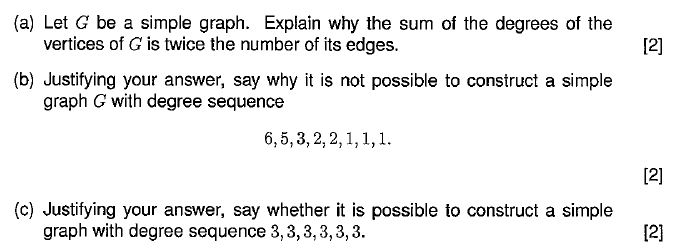
\includegraphics[width=0.7\linewidth]{GraphTheoryQuestion2012}
%
%\end{figure}


%----------------------------------------------------------------%
\newpage
\section*{Question 6}
% 2007 Q8
Given a flock of chickens, between any two chickens one of them is
dominant. A relation, R, is defined between chicken x and chicken y as xRy if x is
dominant over y. This gives what is known as a pecking order to the flock. Home
Farm has 5 chickens: Amy, Beth, Carol, Daisy and Eve, with the following relations:

\begin{itemize}
\item Amy is dominant over Beth and Carol
\item Beth is dominant over Eve and Carol
\item Carol is dominant over Eve and Daisy
\item Daisy is dominant over Eve, Amy and Beth
\item Eve is dominant over Amy.
\end{itemize}

\newpage
\section*{Question 6}
% Digraphs and Relations
% http://staff.scem.uws.edu.au/cgi-bin/cgiwrap/zhuhan/dmath/dm_readall.cgi?page=20

Let $A=\{0,1,2\}$ and $R=\{ (0,0),(0,1),(0,2),(1,1), (1,2), (2,2)\}$
and $S=\{(0,0),(1,1),(2,2)\}$ be 2 relations on A. Show that

\begin{itemize}
\item[(i)] R is a partial order relation.
\item[(ii)] S is an equivalence relation.
\end{itemize}
%---------------------------------------------------------------------------%

%2002 Question 7
Let S be a set and let R be a relation on S
Explain what it means to say thet $\mathcal{R}$ is

\begin{itemize}
\item[(i)] reflexive
\item[(ii)] symmetrix
\item[(iii)] anti-symmetric
\item[(iv)] Transitive
%---------------------------------------------------------------------------%



\end{itemize}


%--------------------------------------------------------------------------- %
\section*{Question 7}
Let the sequence un be defined by the recurrence relation
\[u_{n+1} = u_n + 2n, \mbox{ for n = 1, 2, 3, ...}\]
and let $u_1 = 1$.\\
%\begin{figure}[h!]
%\centering
%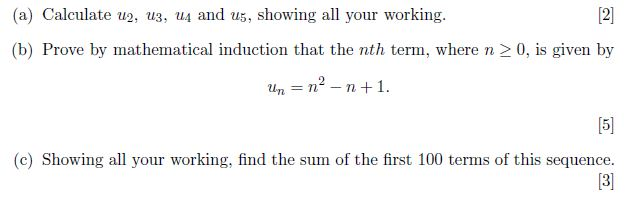
\includegraphics[width=1.11\linewidth]{SeqSerQuestion2005}
%\end{figure}

%---------------------------------------------------------------------------%
% TREES
\newpage
\section*{Question 8}
%\noindent \textbf{(Part A : Spanning Trees -  5 Marks) }\\
%\begin{figure}[h!]
%\centering
%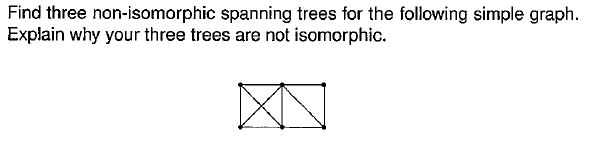
\includegraphics[width=1.11\linewidth]{TreesQuestion2012}
%\end{figure}

%Question 8A
%\begin{enumerate}
%\item How many edges are in the spanning tree $T$ ?
%\item What is the sum of the degree sequence of $T$?
%\item Write down all the possible degree sequences for the spanning tree $T$.
%\end{enumerate}
%---------------------------------------------------------------------------%


\noindent \textbf{(Part B :Binary Search Trees -  5 Marks) }\\
Suppose a database, comprised of 30,000 internal nodes, is structured as a Binary Search Tree.

\begin{enumerate}[(i)]
\item What is the Key of the Root node?
\item What are the keys of the nodes at level 1?
\item For the nodes at level 1, how many subtrees are there?
%\item State which nodes are in the substrees of the level 1 nodes?
\item How many nodes are the between the root (level 0) and level 4. ]
%(Hint: use a summation theorem mentioned in session 7
\item What is the maximum number of searchs in this database?
\end{enumerate}

%============================================================================%

\section*{ Question 9 }
Given S is the set of all 5 digit binary strings, E is the set of a 5 digit
binary strings beginning with a 1 and F is the set of all 5 digit binary strings ending
with two zeroes.
\begin{itemize}
\item[(a)] Find the cardinality of S, E and F.
\item[(b)] Draw a Venn diagram to show the relationship between the sets S, E and F.
Show the relevant number of elements in each region of your diagram.
\end{itemize}

\begin{itemize}
\item A college teaches courses in the following subjects areas: mathematics, computing and statistics.
\item Students in the college may choose their courses from these three subject areas.
\item Students are not obliged to take courses from these three subject areas, and may instead take courses in other subject areas. 
\item  Let the subject areas be represented by the letters \textbf{M} for mathematics, \textbf{C} for computing and \textbf{S} for statistics. \item Draw a labelled Venn diagram showing the areas \textbf{M}, \textbf{C}, and \textbf{S} in such a way as to represent the students studying at the college. \item On your diagram show the number of students studying in each region of the Venn diagram.
%===================%
\begin{itemize}
\item Currently 600
students are enrolled in the college. 
\item 300 students are taking mathematics courses.
\item 120 student are taking statistics courses.
\item 380 students are taking computing courses. 
\item 40 students study courses from all three subject
areas. 
\item 200 mathematics students are taking computing courses as well. \item 60 computing students
are also takings statistics courses. \item  70 statistics students are also taking mathematics course.
\end{itemize}
\end{itemize}

%==============%
\begin{itemize}
\item[(i)] How many students study none of these courses at all?
\item[(ii)] How many students are taking mathematics courses but not computing or statistics courses.
\item[(iii)] How many students study courses from precisely two of these subject
areas?

\end{itemize}
\newpage
%===========================================================%
\section*{Question 10}
%%--------------------------------------------%
%\noindent \textbf{Part A : Matrix Operations - 4 Marks}\\ 
%\begin{figure}[h!]
%\centering
%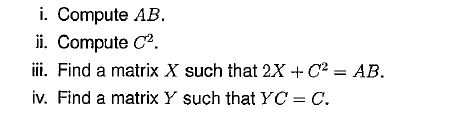
\includegraphics[width=1.11\linewidth]{MatrixQuestion2012}
%
%\end{figure}


%--------------------------------------------%
\noindent \textbf{Part B : Gaussian Elimination - 5 Marks}\\ 
\begin{itemize}
\item[(i)] Say whether or not the graphs they represent are isomorphic.
\item[(ii)] Calculate $A^2$ and $A^4$ and say what information each gives about the graph
corresponding to A. [6]
\end{itemize}
%===========================================%
\begin{itemize}
\item[(i)] Write down the augmented matrix for the following system of equations.
\[2x + y - z = 2\]
\[x - y + z = 4\]
\[x + 2y + 2z = 10\]
\item[(ii)] Use Gaussian elimination to solve the system. 
\end{itemize}
%=========================================================================================== %


%-------------------------------------------------------------------------%
\newpage

\end{document}
